\documentclass{article}
\usepackage{tikz} 
\usepackage[utf8]{inputenc}
\usepackage{amsmath}
\usepackage{listings}
\usepackage{amsfonts}
\usepackage{amssymb}
\usepackage{tabularx}
\usepackage{enumitem}
\usepackage{algorithm}% http://ctan.org/pkg/algorithm
\usepackage[noend]{algpseudocode}% http://ctan.org/pkg/algorithmicx
\usepackage{tikz}
\usepackage{graphicx}
\usepackage{standalone}

\usepackage{subcaption}
\usepackage{multicol,caption}
\usepackage{geometry}
 \geometry{
 a4paper,
 total={210mm,297mm},
 left=20mm,
 right=20mm,
 top=20mm,
 bottom=20mm,
 }

\usetikzlibrary{arrows,positioning,shapes} 
\pgfarrowsdeclarecombine{ring}{ring}{}{}{o}{o}
\thispagestyle{empty}
\DeclareMathOperator{\ringarrow}{\raisebox{0.5ex}{\tikz[baseline]{\draw[ring->](0,0)--(2em,0);}}}

\definecolor{talk}{HTML}{729FCF}
\definecolor{talk2}{HTML}{E8A753}
\definecolor{grey}{HTML}{DBDCDD}
\renewcommand{\vec}[1]{\boldsymbol{#1}}
\tikzset{
    %Define standard arrow tip
    >=stealth',
    %Define style for boxes
    observed/.style={
   	circle,
   	rounded corners,
   	draw=black, thick,
   	minimum width=2.3em,
   	minimum height=2.3em,
   	font=\footnotesize,
   	text centered,
   	fill=talk!50
   },
   latent/.style={
   	circle,
   	rounded corners,
   	draw=black, thick, dashed,
   	minimum width=2.2em,
   	minimum height=2.2em,
   	font=\footnotesize,
   	text centered
   },
    % Define arrow style
    pil/.style={
           o->,
           thick,
           shorten <=2pt,
           shorten >=2pt,},
    sh/.style={ shade, shading=axis, left color=red, right color=green,
    shading angle=45 },
observedrect/.style={
	rectangle,
	rounded corners,
	draw=black, thick,
	minimum width=3em,
	minimum height=1.5em,
	font=\footnotesize,
	text centered,
	fill=talk2!50
}  
}
   
\begin{document}
\pagestyle{empty}
\def\ci{\perp\!\!\!\perp} % from Wikipedia
\begin{figure}[ht]
	\centering
	\begin{subfigure}[t]{0.29\textwidth}
		\centering
		\caption{$\vec{X}$ causes $\vec{Y}$}
		\label{fig:context-graph-causal}
		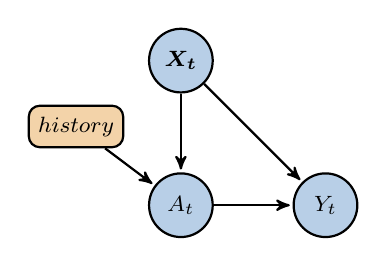
\begin{tikzpicture}[->,>=stealth',shorten >=1pt,auto,node distance=1cm,
		thick,main node/.style={observed},lt/.style={latent},history/.style={observedrect}]
		\node[main node](4){$\vec{X_t}$};
		\node[main node, below=of 4](3){$A_t$};
		\node[main node, right=of 3](2){$Y_t$};
		\node[history,left=of 3, xshift=.7cm,yshift=1cm](5){$history$};
		\path[every node/.style={font=\sffamily\small}]
		(3) edge (2)
		(4) edge (2) edge (3)
		(5) edge (3);
		\end{tikzpicture} 
	\end{subfigure}
	\begin{subfigure}[t]{0.29\textwidth}
		\centering
		\caption{$\vec{X}$ and $\vec{Y}$ are confounded}
		\label{fig:context-graph-confounded}
		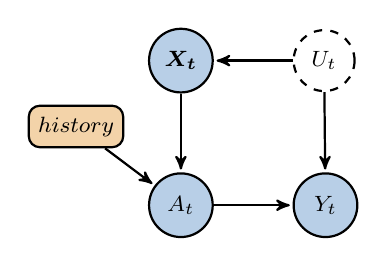
\begin{tikzpicture}[->,>=stealth',shorten >=1pt,auto,node distance=1cm,
		thick,main node/.style={observed},lt/.style={latent},history/.style={observedrect}]
		\node[main node](4){$\vec{X_t}$};
		\node[main node, below=of 4](3){$A_t$};
		\node[main node, right=of 3](2){$Y_t$};
		\node[lt,right=of 4](1){$U_t$};
		\node[history,left=of 3, xshift=.7cm,yshift=1cm](5){$history$};
		\path[every node/.style={font=\sffamily\small}]
		(3) edge (2)
		(4) edge (3)
		(1) edge (2) edge (4)
		(5) edge (3);
		\end{tikzpicture} 
	\end{subfigure}
	\begin{subfigure}[t]{0.29\textwidth}
		\centering
		\caption{$\vec{Y}$ causes $\vec{X}$}
		\label{fig:context-graph-anti-causal}
		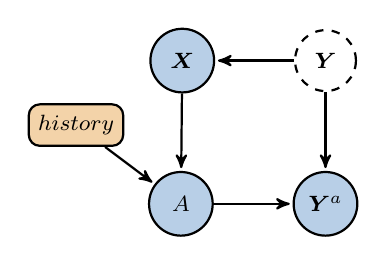
\begin{tikzpicture}[->,>=stealth',shorten >=1pt,auto,node distance=1cm,
		thick,main node/.style={observed},lt/.style={latent},history/.style={observedrect}]
		%nodes
		\node[lt](1){$\vec{Y}$};
		\node[main node, below=of 1](2){$\vec{Y}^a$};
		\node[main node, left=of 2](3){$A$};
		\node[main node, left=of 1](4){$\vec{X}$};
		\node[history,left=of 3, xshift=.7cm,yshift=1cm](5){$history$};
		\path[every node/.style={font=\sffamily\small}]
		(1) edge (4)
		(3) edge (2)
		(1) edge (2)
		(5) edge (3)
		(4) edge (3);
		\end{tikzpicture} 
	\end{subfigure}
\end{figure}

\end{document}